\documentclass{beamer}
\usepackage[utf8]{inputenc}
\usepackage[ngerman]{babel}
\usepackage{graphicx}
\usepackage{listings}

\lstset{
	basicstyle=\ttfamily,
	frame=single,
	numbers=left,
	language=C,
	breaklines=true,
	breakatwhitespace=true,
	postbreak=\hbox{$\hookrightarrow$ },
	showstringspaces=false,
	tabsize=4
}

\renewcommand*{\lstlistlistingname}{Listingverzeichnis}



\usetheme{CambridgeUS}
\usecolortheme{dolphin}
\title{Parallele Programmierung - Solitaire Chess}
\author{Kira Duwe - Enno Zickler}
\institute{DKRZ- UHH}
\date{\today}
\begin{document}

\begin{frame}
\titlepage
\end{frame}


\begin{frame}{Spielregeln}
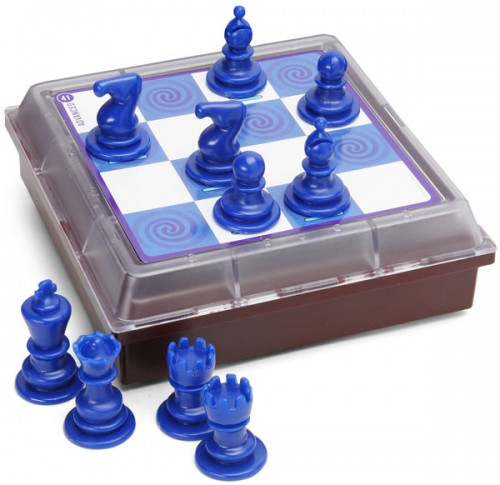
\includegraphics[scale=0.2]{solitaire}
\begin{itemize}

	\item Figuren ziehen nach Schachregeln
	\item pro Zug eine Figur ziehen, um eine andere zu schlagen
	\item 4 x 4 - Brett
	\item 10 Figuren : 2 x Bauer, Türme, Springer, Läufer; 1 x König und Dame
	\item Ziel: eine einzige Figur bleibt übrig

\end{itemize}
\end{frame}

\begin{frame}{Fragestellungen}
Vorhaben
\begin{itemize}

	\item Welche Startpositionen sind lösbar? (mit variierender Figurenanzahl)
	\item Mögliche Erweiterungen: 
	\begin{itemize}
	\item größeres Spielbrett 
	\item andere Brettform
	\item In wie viel Zügen ist ein Spiel lösbar? 
	\item Wie viele unterschiedliche zum Ziel führende Zugmöglichkeiten gibt es?
	\end{itemize}
\end{itemize}

Ergebnis
\begin{itemize}
	\item Wie viele Spielbretter sind lösbar
	\item Alle Spielbretter mit 1 bis 10 Figuren
	\item Variable Brettgröße von 1 bis 21 Felder in beliebiger rechteckiger Form
\end{itemize}
\end{frame}


\begin{frame}{Spielbrettdarstellung}
\begin{columns}
\column{.65\textwidth}
	Oktaldarstellung
	\begin{itemize}
		\item 16 Felder * 3 bit = 48 bit
		\item uint64 ist ausreichend
		\item kleiner als Array (16 * 8 bit = 128 bit)
		
		\begin{table}
			\begin{tabular}{|c|c|c|c|}\hline
			 0 &  1 &  0 &  0 \\ \hline
			 0 &  5 &  6 &  0 \\ \hline
			 4 &  2 &  1 & 4 \\ \hline
			 2 &  3 &  0 &  3 \\ \hline
			\end{tabular}
			\caption{Spielbrett 3032 4124 0650 0010}
			\label{table:Tabelle1}
		\end{table}
	\end{itemize}
\column{.35\textwidth}
	Figuren
	\begin{itemize}
		\item 0 = leeres Feld
		\item 1 = Bauer
		\item 2 = Turm
		\item 3 = Läufer
		\item 4 = Springer
		\item 5 = König
		\item 6 = Dame
	\end{itemize}		
\end{columns}
\end{frame}

\begin{frame}{Spielbretterzeugung}
\begin{itemize}
	\item Verschachtelte for-Schleifen, für jede Figur von 0 bis Spielbrettgröße
	\item bei doppelten Figuren sollte die 2. Figur abhängig von der 1. sein
	\item Abschneiden der Schleifendurchläufe, wenn betrachtetes Feld nicht frei
\end{itemize}
\end{frame}


\defverbatim[colored]\Lst{%
\begin{lstlisting}[tabsize=2,frame=single]
for(Dame von 0 bis 16)
	if( Feldfrei)
		for(Koenig von 0 bis 16)
			if( Feldfrei)
				for (Springer1 von 0 bis 16)
					if( Feldfrei)
						for (Springer2 von posSpringer1 bis 16)
							...
								for (Bauer2 von posBauer1 bis 16)
									Spielbrettberechnen
\end{lstlisting}}

\begin{frame}[allowframebreaks]{Spielbretterzeugung}
\Lst
\end{frame}


\begin{frame}{Spielbrettberechnung}
\begin{itemize}
	\item Dynamische Programmierung
	\item Vorherige Lösungen werden wieder verwendet
	\item Erzeugung nach Figurenanzahl (+ for-Schleife)
	\item Berechnung nach Figurenanzahl aufsteigend
	\item Lösungen der vorherigen Ebene müssen bekannt sein
\end{itemize}
\end{frame}


\begin{frame}{Spielbrettberechnung}
\begin{itemize}

	\item Umwandlung in Array für Zugberechnung
	\item Felderweise Überprüfung des gesamten Brettes, ob durch möglichen Zug ein lösbares Brett entsteht
	\item Zugriff auf vorherige Lösungen
	\item Abbruch der Berechnung, wenn Nachfolgebrett als lösbar gespeichert 
\end{itemize}
\end{frame}

\defverbatim[colored]\Lst{%
\begin{lstlisting}[tabsize=2,frame=single]
einser_Bitmaske = 0xffffffffffffffffLL;

// Spielfiguren, geschlagene und schlagende, von Spielbrett loeschen 
// Von der Bitmaske wird "(7 << pos*3)" abgezogen, um an dieser Stelle 0 zu erzeugen 
	
	neues_spielbrett = spielbrett & 
	(einser_Bitmaske - (7 << pos*3) - (7 << neue_pos*3));
	
// nach Schlagen Spielfigur neu  setzen 
	neues_spielbrett += 
	(DarstellungFigur << neue_pos*3);
\end{lstlisting}}

\begin{frame}[allowframebreaks]{Schlagen der Figuren}
\Lst
\end{frame}




\begin{frame}{Größe des Problems}
\begin{columns}
	\column{.45\textwidth}
		\begin{itemize}
			\item 6.7 Milliarden Spielbretter für 4x4
			\item sehr großer Anteil lösbar
				
			\end{itemize}

	\column{.55\textwidth}
	\begin{center}
		\begin{tabular}{|c|r|c|} \hline
		Figuren:  & Anzahl & \% Lösbar:  \\ \hline \hline
		  1 & 96 &  100.00   \\ \hline
		  2 & 4.080 &   50.25   \\ \hline
		  3 & 100.800&   70.95   \\ \hline
		  4 & 1.594.320 &   89.41   \\ \hline
		  5 & 16.773.120&   97.62   \\ \hline
		  6 & 118.198.080&   99.70   \\ \hline
		  7 & 547.747.200&   99.98   \\ \hline
		  8 & 1.589.187.600 &  100.00   \\ \hline
		  9 & 2.594.592.000 &  100.00   \\ \hline
		 10 & 1.816.214.400 &  100.00   \\ \hline \hline
		  Gesamt  & 6.684.411.696 &  99.98   \\ \hline
		
		\end{tabular}
	\end{center}


\end{columns}
\end{frame}

\begin{frame}{Speicherung}
	\begin{itemize}
		\item Abspeichern der Spielbretter in Hashtablle / Hashset
		\item 6.684.411.696 x 64bit x 2 = 855.604.697.088 bit = 106 GByte
		\item Hashset fürt zu Halbierung des Speicherbedarfs
		\item Optimierung durch speichern der nicht lösbaren 
		\item 1.047.721 x 64 bit = 67.054.144 bit = 67 MB 
	\end{itemize}
\end{frame}

\begin{frame}{Output Solitaire-Schach 4x4 auf 8 Knoten mit je 24 Threads}
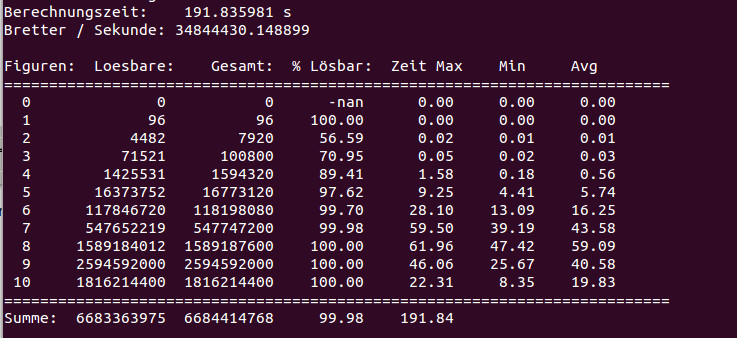
\includegraphics[scale=0.4]{output}
\end{frame}

\begin{frame}{gprof}
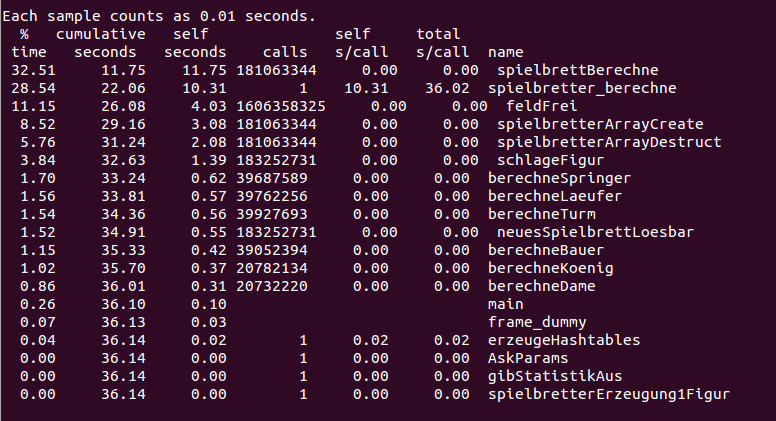
\includegraphics[scale=0.4]{gprof}
\end{frame}

\begin{frame}{MPI-Kommunikation}
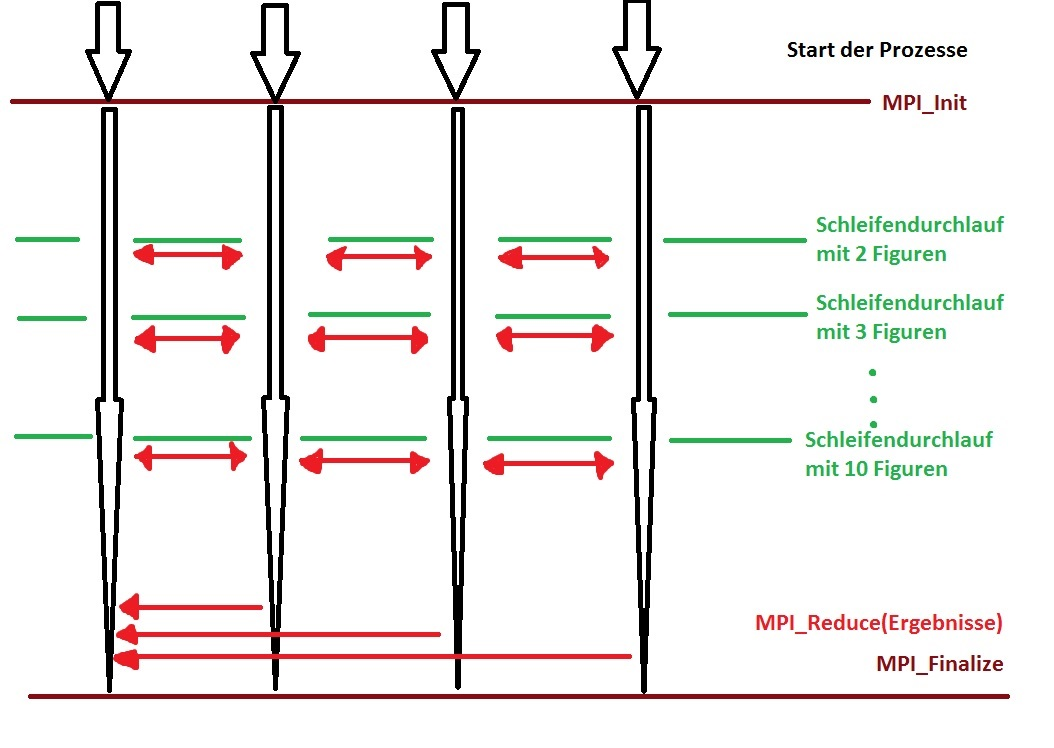
\includegraphics[scale=0.3]{MPI_Kommunikation}
\end{frame}

\begin{frame}{Speedup 4x4-Spielbrett mit 24 Thread/Knoten}
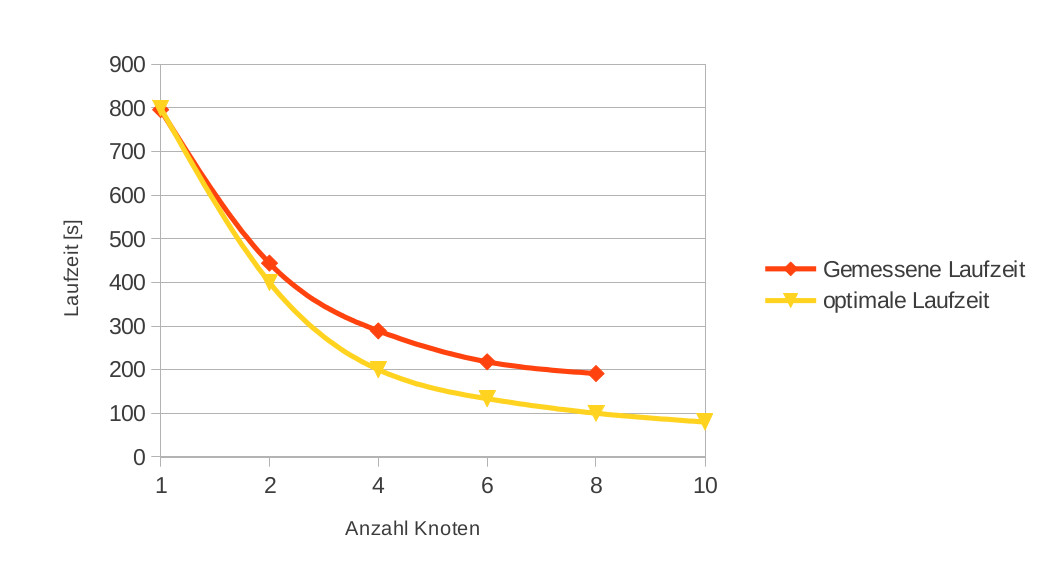
\includegraphics[scale=0.3]{speedup}
\end{frame}

\begin{frame}{Vampirtrace - Profile}
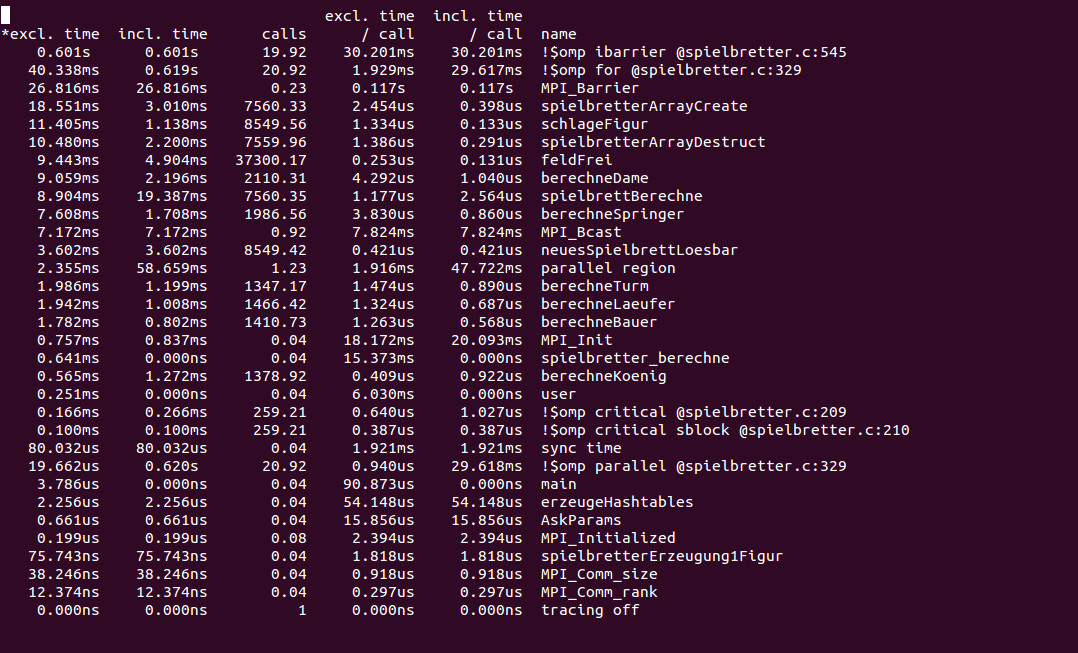
\includegraphics[scale=0.3]{vampirtrace-prof}
\end{frame}



% Include all the stuff for OS
%\include{betriebssysteme}

% Include all the stuff for Linux
%\include{linuxintro}

\end{document}
